\section{方法描述}

\subsection{图文实体}
\label{sec:4_entities}
\begin{figure}[!htbp]
    \centering
    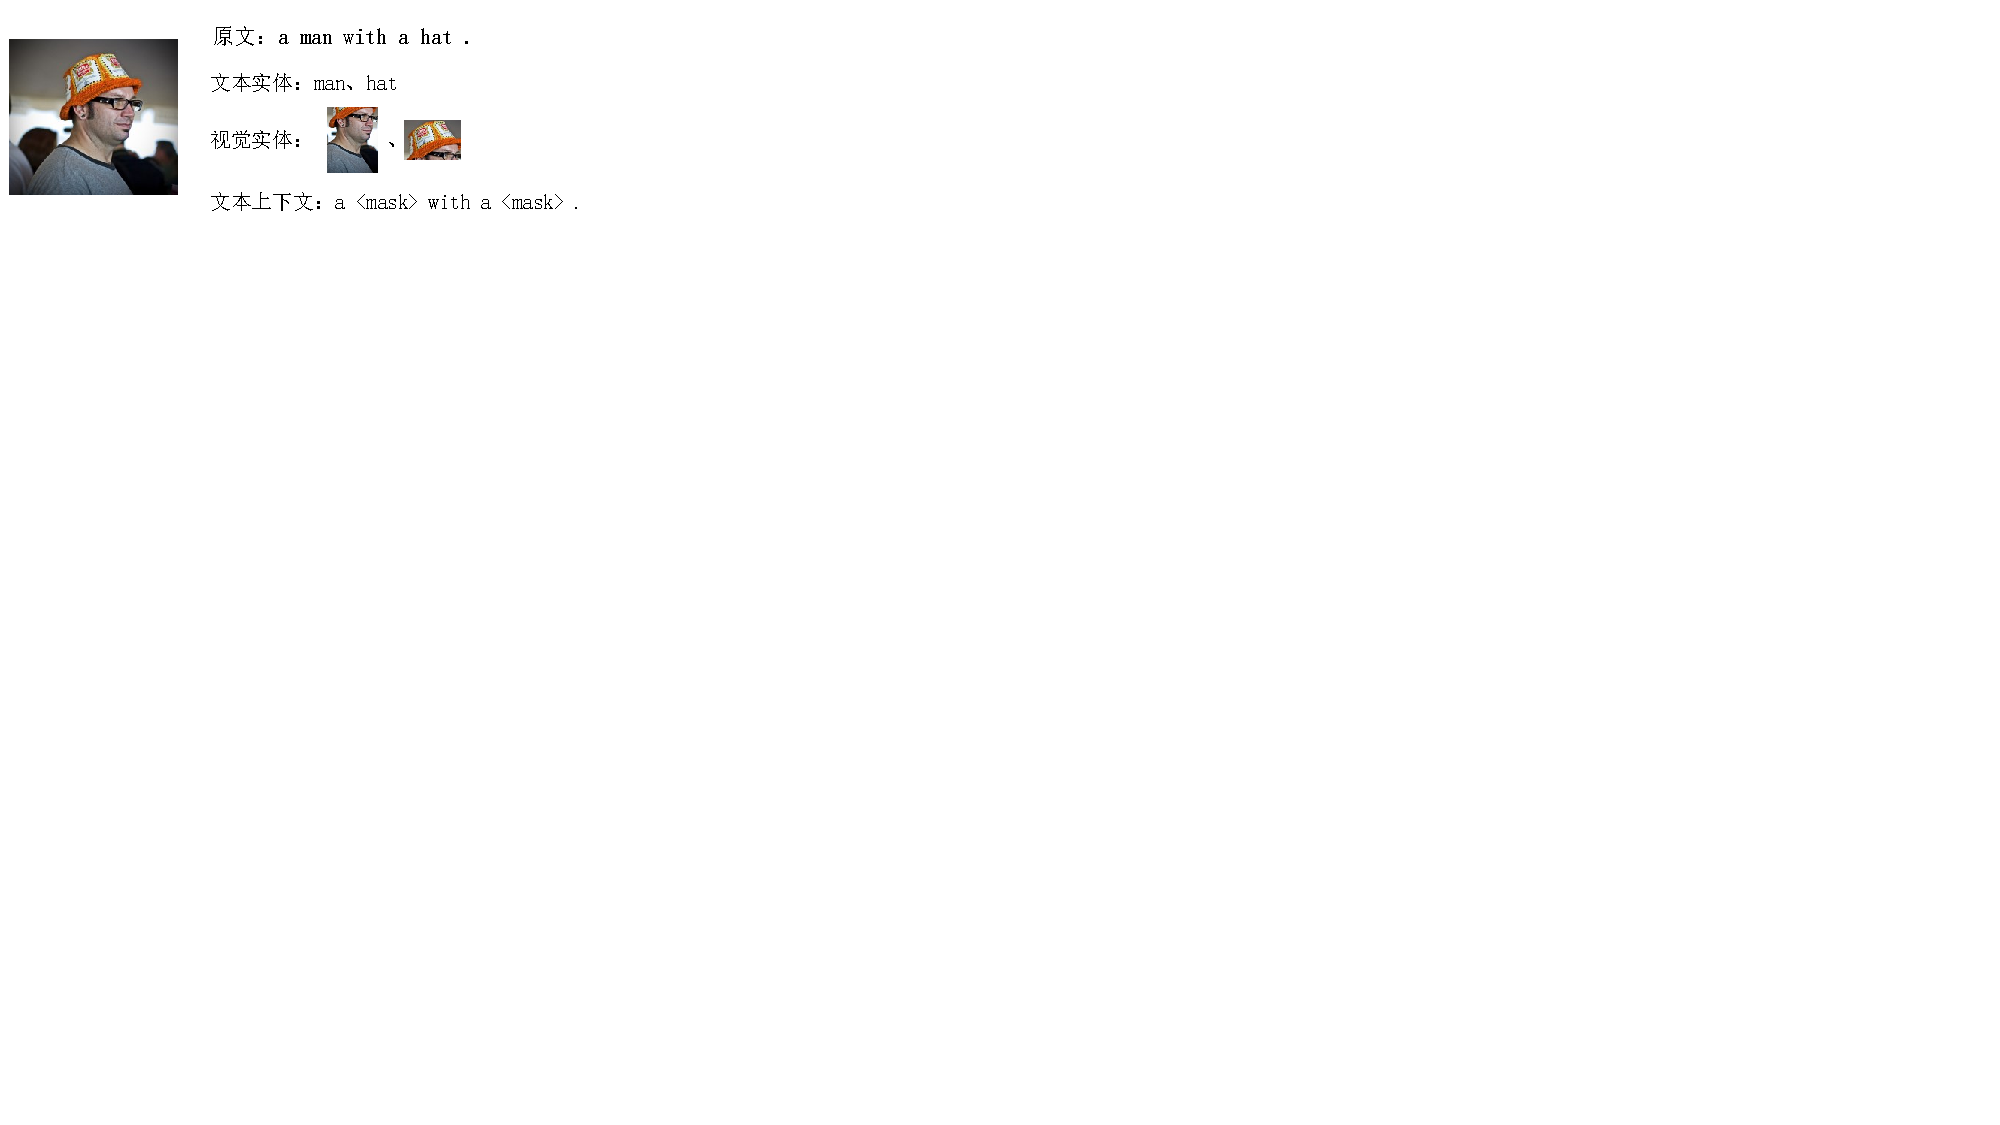
\includegraphics{Img/fig_4_definations.pdf}
    \bicaption{图文实体}{Visual entities and textual entities}
    \label{fig:4_definations}
\end{figure}
为了更方便地对本章所提的CER方法进行介绍,首先需要对CER方法作用到的图片视觉目标和文本中的作用目标进行更恰当的定义:

(1){\sffamily 文本实体:}输入的源语言句子$X=\{t_1,t_2,\cdots,t_N\}$中,在对应图片有对应视觉目标的名词$t_a,t_b,\cdots$为文本实体(textual entity),$T=\{t_a,t_b,\cdots\}$为它们的集合。如图\ref{fig:4_definations}所示,名词“man”和“hat”在图片中均有与其对应的视觉目标,因此符合文本实体的定义。从该定义同样可知,文本实体与上一章\ref{sec:3_entity_replacement}小节所介绍的词实体本质上是相同的。本章不再将名词短语划为实体范畴进行考虑,只针对名词融合视觉信息。

(2){\sffamily 视觉实体:}文本实体在对应图片$I$中的对应视觉目标${e_a,e_b,\cdots}$为视觉实体(visual entity),$E=\{e_a,e_b,\cdots\}$为它们的集合。图\ref{fig:4_definations}中的“男人”和“帽子”分别是名词实体“man”和“hat”在图片中对应的视觉目标,因此是视觉实体。

(3){\sffamily 文本非实体:}在源语言句子中,所有非文本实体的单词均可称为文本非实体(textual none-entity)。$\tilde{X}=X-T$代表它们的集合、文本上下文或退化文本。例如图\ref{fig:4_definations}中,文本上下文中除“<mask>”外均为文本非实体。

\subsection{跨模态编码}
图【】展示了CER模型与NMT模型相融合的简化过程,其中包含了跨模态编码、跨模态实体重构以及NMT三个主要任务。跨模态编码负责在进行实体重构之前将视觉信息与文本信息编码融合。所编码的信息包含实体重构主要依赖的三部分:

%\begin{itemize}
%\item
(1){\sffamily 跨模态实体:}其中实体重构主要依赖于跨模态实体所提供的具体信息。如图【】所示,文本实体$t_1$的重构主要依赖于视觉实体$e_1$,视觉实体$e_1$的重构也主要依赖于文本实体$t_1$。

%\item
(2){\sffamily 文本上下文:}本文所用文本上下文为经过退化的文本$\tilde{X}$。例如图【】中进行实体重构时,文本上下文为“A <M> with a <M>”,其中“<M>”代表将实体词所对应的位置删除并保留该位置空缺。文本上下文与跨模态实体共同组成文本的完整语义。在进行视觉实体重构时,模型的输入由文本上下文和文本实体共同组成,即原文本$X$。在进行文本实体重构时,模型的输入是文本上下文和视觉实体所组成的多模态混合序列$Z$。在进行文本非实体的重构时,模型的输入同样是多模态混合序列,但是需要将待重构的非实体词利用掩码词“<M>”替换掉,形成$\tilde{Z}$。跨模态实体与文本上下文组合重构实体的方式,既能保证重构实体时具备充足的语义信息,又能充分利用到自注意力机制的特性使实体与文本上下文建立良好的语义关系。

%\item
(3){\sffamily 实体对齐关系:}为了避免让模型完成较为困难的跨模态实体关系对齐,本文采用直接替换对应位置向量表示的方式。例如图2中重构文本实体$t_1$时,将输入序列中的对应位置直接替换为视觉实体的向量表示${\boldsymbol{e}_1}$。

\subsection{跨模态实体重构}
{\sffamily 视觉实体重构}

视觉实体重构(Visual entity reconstruction,VER)依赖于原文本$X$。例如图2中,“A man with a hat”为重构视觉实体时模型的输入序列,此时图中输入到模型中的是5个圆形空心词向量。该句子经过$L$层的编码器进行文本编码,再利用$L$层视觉实体解码器解码出与文本实体$\{t_1,t_5\}$相对应的视觉实体$\{e_1,e_5\}$。由于文本无法完整的描述图片,只是针对图片中的个别属性的描述,由文本直接还原像素级的图片或图片中的视觉实体几乎是不可能的。因此本文仅尝试生成与视觉实体最相近的向量表示$\{{\boldsymbol{e}_1},{\boldsymbol{e}_5}\}$。其中,$X$经过如下编码过程:
\begin{equation}
H_X^L={\rm{MHSAtt_{enc}}}(X, X, X)
\end{equation}
得到编码后的隐层表示$H_X^L=\{{\boldsymbol{h}_1^l},{\boldsymbol{h}_2^l},\cdots,{\boldsymbol{h}_N^l}\}$,其中$L$表示编码器层数,${\rm MHSAtt_{enc}}(\cdot)$为$L$层多头自注意力编码器。然后经过如下解码过程:
\begin{equation}
H_X^{2L}={\rm{MHSAtt_{dec}}}(H_X^L, H_X^L, H_X^L)
\end{equation}
得到$H_X^{2L}=\{{\boldsymbol{h}_1^{2l}},{\boldsymbol{h}_2^{2l}},\cdots,{\boldsymbol{h}_N^{2l}}\}$,${\rm MHSAtt_{dec}}(\cdot)$为与${\rm MHSAtt_{enc}}(\cdot)$具有相同结构的视觉实体解码器。然后利用$H_X^{2L}$生成与$\{{\boldsymbol{e}_a},{\boldsymbol{e}_b},\cdots\}$接近的向量表示,文本采用与文献${[5]}$相近的方式实现该过程:
\begin{equation}
\mathcal{L}_{\rm{VER}}(\theta, \varphi)=
    \frac{1}{{\vert}E{\vert}}
    \mathop{\sum}_{j{\neq}i} {\max}\{0, \varepsilon - {\rm{cos}}\left( {\boldsymbol h_i^{2l}}, {\boldsymbol e_j} \right) + {\rm{cos}}\left( {\boldsymbol h_i^{2l}}, {\boldsymbol e_i} \right)\}
\end{equation}
%\onecolumn
%\input{docs/model_pic.tex}
%\begin{multicols}{2}
其中$i,j{\in}\{a,b,\cdots\}$,$\theta$为文本编码器参数,$\varphi$为视觉实体解码器的参数,${\rm{cos}}(\cdot,\cdot)$计算向量间的余弦相似度,$\varepsilon$为最小边缘常量。显然,优化$L_{\rm{VER}}(\theta,\varphi)$能够缩减${\boldsymbol{h}_i^{2l}}$与正样本${\boldsymbol{e}_i}$之间的余弦距离,增加与负样本${\boldsymbol{e}_j}$之间的余弦距离。


{\sffamily 文本实体重构}

文本实体重构(Textual entity reconstruction,TER)依赖于由文本上下文$\tilde{X}$和视觉实体E组合成的多模态混合序列:
\begin{equation}
Z={\rm{Combine}} \left( \tilde{X}, E \right)
\end{equation}
如图2所示,输入的文本上下文“A <M> with a <M>”与视觉实体$\{e_1,e_5\}$组合成多模态混合序列$Z=$“A $e_1$ with a $e_5$”,此时输入到模型中的是三个圆形空心词向量和两个标记“V”的圆形视觉特征。多模态混合序列经过编码器进行跨模态编码后,得到序列的跨模态表示:
\begin{equation}
H_Z^L={\rm{MHSAtt_{enc}}} \left( Z, Z, Z \right)
\end{equation}
其中,$H_Z^L=\{{\boldsymbol{h}_1^l},{\boldsymbol{h}_2^l},\cdots,{\boldsymbol{h}_N^l}\}$。然后依据对应位置的隐层表示生成文本实体,在图2中为两个标记“V”矩形隐层表示${\boldsymbol{h}_2^l}$和${\boldsymbol{h}_5^l}$,该过程需要优化以下损失函数:
\begin{equation}
\mathcal{L}_{\rm{TER}} (\theta, \vartheta) =
    \frac{1}{{\vert}T{\vert}}
    \mathop{\sum}_{x_i \in T}
    {\rm{OH}} \left( x_i \right)
    {\rm log}{\ }{\rm p} \left( Z {\vert} \theta, \vartheta \right)
\end{equation}
\begin{equation}
{\log}{\ }{\rm p} \left( Z {\vert} \theta, \vartheta \right) =
    {\rm{g}} \left( {\boldsymbol h_i^l} \vert \vartheta \right)
\end{equation}
其中${\rm{OH}}\left(x_i\right)$代表$x_i$的独热编码(One-hot,OH)表示,$\vartheta$为生成器(Generator)参数,生成器${\rm{g}}\left(\cdot\right)$将位置$i$处的隐层向量${\boldsymbol{h}_i^l}$映射并得到词表中每个词的预测概率$p$。

{\sffamily 文本非实体重构}

文本非实体重构(Textual none-entity reconstruction,TNER)方法与文本实体重构方法相似,区别在于非实体重构的目的是使视觉实体与文本上下文进行充分的句子级语义融合,而实体的重构方法更侧重实体在两个模态之间的实体级语义融合。文本非实体的输入同样是文本上下文$\tilde{X}$和视觉实体$E$组合成的多模态混合序列,但是在$\tilde{X}$中除对实体的位置进行退化还要将待重构的非实体词退化。例如图2中,当选中对非实体词“A”进行重构时,模型所输入的多模态混合序列为$Z=$“<M> $e_1$ with a $e_5$”,此时输入到模型中的是一个标记“N”的圆形词向量代表“<M>”、两个圆形空心词向量和两个标记“V”的圆形视觉特征。损失函数如下:
一个标记``N''的圆形词向量代表``$\langle$M$\rangle$''、两个圆形空心词向量和两个标记``V''的圆形视觉特征. 损失函数如下:
\begin{equation}
\mathcal{L}_{\rm{TNER}}(\theta, \vartheta) =
    \frac{1}{{\vert}\tilde{T}{\vert}}
    \mathop{\sum}_{x_i \in \tilde{T}}
    {\rm{OH}} \left( x_i \right)
    {\rm log}{\ }{\rm p} \left( \tilde{Z} {\vert} \theta, \vartheta \right)
\end{equation}
其中$\tilde{T}$代表待重构的非实体词集,并有$\tilde{T}\subseteq X-T$。在图2中用于预测非实体词“A”的隐层为一个标记“N”的矩形隐层表示${\boldsymbol{h}_1^l}$。

本文采用随机选取的方式选择待重构的非实体词。在执行TNER任务时,每个文本中的非实体词有$30\%$的概率会被选择到。该概率与所采用数据集中实体词占$32.6\%$的比例相近。

{\sffamily CER联合训练}

联合以上所有重构方法的目标函数,可得到本文所提CER方法的联合损失函数为:
\begin{equation}
\mathcal{L}_{\rm{CER}} \left( \theta, \varphi, \vartheta \right) = \alpha \mathcal{L}_{\rm{VER}} \left( \theta, \varphi \right) + \beta \mathcal{L}_{\rm{TER}} \left( \theta, \vartheta \right) + \gamma \mathcal{L}_{\rm{TNER}} \left( \theta, \vartheta \right)
\end{equation}
其中,$\alpha$、$\beta$和$\gamma$为控制三种重构方法训练比例的超参数。值得注意的是,本文没有设置利用纯文本上下文$\tilde{X}$重构文本词的方案。这是因为该方案与一般的预训练方法相似,用于建立纯文本的语言模型。而机器翻译模型的编码端本身就是一个很好的纯文本语言模型,因此不必再设置纯文本的重构方案。

\subsection{与机器翻译相结合}
构建CER模型的目的是辅助翻译模型提升翻译质量。本文采用多任务学习方法将CER模型中的跨模态编码器与NMT模型的文本编码器进行参数共享,从而实现将跨模态信息融合到NMT模型的目的。NMT任务所要优化的目标函数为:
\begin{equation}
\mathcal{L}_{\rm{NMT}} \left( \theta, \psi, \vartheta \right) =
    -\mathop{\sum}_j^M {\rm log}{\ }{\rm P} \left(y_j \vert y_{<j}, X \vert \theta, \psi, \vartheta \right)
\end{equation}
其中$Y=\{y_1,y_2,\cdots,y_M\}$为目标语言的文本序列。将式(13)与CER模型的损失函数式(12)相结合得到联合目标函数为:
\begin{equation}
\mathcal{L} \left( \theta, \psi, \varphi, \vartheta \right) = \omega\mathcal{L}_{\rm{NMT}} \left( \theta, \psi, \vartheta \right) + \left( 1-\omega \right) \mathcal{L}_{\rm{CER}} \left( \theta, \varphi, \vartheta \right)
\end{equation}
其中,用超参数$\omega$调节NMT模型与CER模型的训练比例。